% Overview of the multi-source federated framework, as a standalone figure.
% Compile on its own (pdflatex, xelatex or lualatex) to FL_structure.pdf and put the PDF into Figures/; main.tex
% includes Figures/FL_structure.pdf at \linewidth (the drawing is ~17.3 cm wide, the CVPR text width 17.5 cm, so the
% fonts keep their size). Caption and label are in main.tex.
\documentclass[10pt,border=2pt]{standalone}
\usepackage{iftex}
\ifPDFTeX
  \usepackage{times}          % the text font of cvpr.sty
\else
  \usepackage{fontspec}       % xelatex/lualatex: the same Times design, loaded by file name
  \setmainfont{texgyretermes}[Extension=.otf, UprightFont=*-regular, BoldFont=*-bold, ItalicFont=*-italic,
    BoldItalicFont=*-bolditalic]
\fi
\usepackage{amsmath,amssymb}
\usepackage{tikz}
\usetikzlibrary{arrows.meta,calc}

\definecolor{cShared}{RGB}{52,101,164}
\definecolor{cLocal}{RGB}{230,126,34}
\definecolor{cInput}{RGB}{142,68,173}
\definecolor{cRestat}{RGB}{39,150,90}
\definecolor{cServer}{RGB}{44,62,80}

\begin{document}
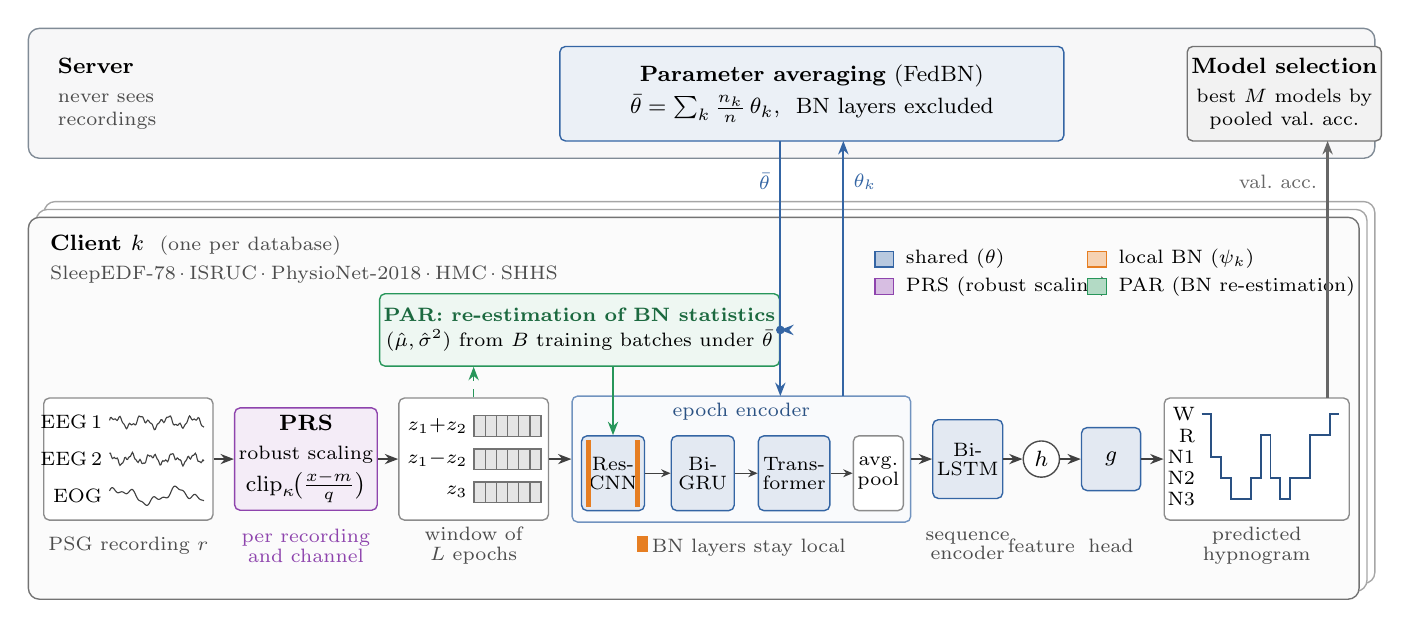
\begin{tikzpicture}[
    font=\footnotesize, line width=0.5pt, >={Stealth[length=1.7mm,width=1.3mm]},
    blk/.style={draw, rounded corners=2pt, align=center, inner sep=1.5pt},
    net/.style={blk, draw=cShared, fill=cShared!14, font=\scriptsize},
    ann/.style={font=\scriptsize, text=black!70, align=center},
    flow/.style={->, black!75},
    encflow/.style={-{Stealth[length=1.2mm,width=1.0mm]}, black!75},
    comm/.style={->, line width=0.8pt},
  ]
  % ------------------------------------------------------------------ server
  \draw[rounded corners=4pt, draw=cServer!60, fill=cServer!4] (0,5.6) rectangle (17.1,7.25);
  \node[align=left, anchor=west] at (0.25,6.42)
    {\textbf{Server}\\[1pt]{\scriptsize\color{black!70}never sees}\\[-1pt]{\scriptsize\color{black!70}recordings}};
  \node[blk, draw=cShared, fill=cShared!10, minimum width=6.4cm, minimum height=1.2cm] (S1) at (9.95,6.42)
    {\textbf{Parameter averaging} (FedBN)\\[2pt]
     $\bar\theta=\sum_{k}\frac{n_k}{n}\,\theta_k$, \ BN layers excluded};
  \node[blk, draw=black!55, fill=black!5, minimum width=2.0cm, minimum height=1.2cm] (S3) at (15.95,6.42)
    {\textbf{Model selection}\\[1pt]{\scriptsize best $M$ models by}\\[-1pt]{\scriptsize pooled val.\ acc.}};

  % ------------------------------------------------------------------ client k (stack of K clients)
  \foreach \off in {0.2,0.1}
    \draw[rounded corners=4pt, draw=black!35, fill=white] (\off,\off) rectangle (16.9+\off,4.85+\off);
  \draw[rounded corners=4pt, draw=black!55, fill=black!1.5] (0,0) rectangle (16.9,4.85);
  \node[anchor=north west, align=left] at (0.15,4.75)
    {\textbf{Client $k$} \ {\scriptsize\color{black!70}(one per database)}\\[1pt]
     {\scriptsize\color{black!70}SleepEDF-78\,\textperiodcentered\,ISRUC\,\textperiodcentered\,PhysioNet-2018%
      \,\textperiodcentered\,HMC\,\textperiodcentered\,SHHS}};
  % legend (2 x 2)
  \foreach \col/\txt/\lx/\ly in {cShared/shared ($\theta$)/10.75/4.32, cLocal/local BN ($\psi_k$)/13.45/4.32,
                                 cInput/PRS (robust scaling)/10.75/3.97, cRestat/PAR (BN re-estimation)/13.45/3.97} {
    \fill[\col!35, draw=\col] (\lx,\ly-0.1) rectangle ++(0.24,0.2);
    \node[anchor=west, font=\scriptsize] at (\lx+0.27,\ly) {\txt};
  }

  % ---- (A) recording
  \node[blk, draw=black!45, fill=white, minimum width=2.15cm, minimum height=1.55cm] (A) at (1.27,1.78) {};
  \foreach \yy/\lab/\fr/\amp/\ph in {2.25/EEG\,1/1/0.10/0, 1.78/EEG\,2/1.25/0.09/70, 1.31/EOG/0.45/0.14/20} {
    \node[anchor=east, font=\scriptsize, inner sep=1pt] at (0.98,\yy) {\lab};
    \draw[black!75, line width=0.4pt] plot[domain=0:1.2, samples=100]
      (\x+1.03, {\yy + \amp*(0.55*sin(\fr*1100*\x+\ph) + 0.3*sin(\fr*2900*\x+40+\ph) + 0.15*sin(\fr*6100*\x+10))});
  }
  \node[ann] at (1.27,0.68) {PSG recording $r$};

  % ---- (B) robust scaling
  \node[blk, draw=cInput, fill=cInput!10, minimum width=1.7cm, minimum height=1.3cm] (B) at (3.525,1.78)
    {\textbf{PRS}\\[1pt]{\scriptsize robust scaling}\\[2pt]$\mathrm{clip}_\kappa\!\big(\frac{x-m}{q}\big)$};
  \node[ann, text=cInput] at (3.525,0.68) {per recording\\[-1pt]and channel};

  % ---- (C) window of L epochs
  \node[blk, draw=black!45, fill=white, minimum width=1.9cm, minimum height=1.55cm] (C) at (5.655,1.78) {};
  \foreach \yy/\lab in {2.2/{$z_1{+}z_2$}, 1.78/{$z_1{-}z_2$}, 1.36/{$z_3$}} {
    \node[anchor=east, font=\scriptsize, inner sep=1pt] at (5.62,\yy) {\lab};
    \draw[draw=black!55, fill=black!10] (5.66,\yy-0.13) rectangle (6.51,\yy+0.13);
    \foreach \ee in {1,...,5} \draw[black!55] (5.66+0.142*\ee,\yy-0.13) -- ++(0,0.26);
  }
  \node[ann] at (5.655,0.68) {window of\\[-1pt]$L$ epochs};

  % ---- (D) epoch encoder; the gaps between its modules leave room for visible arrows
  \node[blk, draw=cShared!70, fill=cShared!3, minimum width=4.3cm, minimum height=1.6cm] (D) at (9.055,1.78) {};
  \node[font=\scriptsize, text=cShared!80!black] at (9.055,2.38) {epoch encoder};
  \node[net, minimum width=0.8cm, minimum height=0.95cm] (D1) at (7.425,1.6) {Res-\\[-1pt]CNN};
  \fill[cLocal] ($(D1.south west)+(0.06,0.06)$) rectangle ($(D1.north west)+(0.13,-0.06)$);
  \fill[cLocal] ($(D1.south east)+(-0.13,0.06)$) rectangle ($(D1.north east)+(-0.06,-0.06)$);
  \node[net, minimum width=0.8cm, minimum height=0.95cm] (D2) at (8.565,1.6) {Bi-\\[-1pt]GRU};
  \node[net, minimum width=0.84cm, minimum height=0.95cm] (D3) at (9.725,1.6) {Trans-\\[-1pt]former};
  \node[blk, draw=black!45, fill=white, font=\scriptsize, minimum width=0.62cm, minimum height=0.95cm] (D4)
    at (10.795,1.6) {avg.\\[-1pt]pool};
  \draw[encflow] (D1) -- (D2); \draw[encflow] (D2) -- (D3); \draw[encflow] (D3) -- (D4);
  \node[ann] at (9.055,0.68) {\textcolor{cLocal}{\rule{4pt}{6pt}}\,BN layers stay local};

  % ---- (E) sequence encoder, (F) feature, (G) head
  \node[net, minimum width=0.85cm, minimum height=1.0cm] (E) at (11.93,1.78) {Bi-\\[-1pt]LSTM};
  \node[ann] at (11.93,0.68) {sequence\\[-1pt]encoder};
  \node[circle, draw=black!70, fill=white, inner sep=1.2pt, minimum size=0.46cm] (F) at (12.865,1.78) {$h$};
  \node[ann] at (12.865,0.68) {feature};
  \node[net, font=\footnotesize, minimum width=0.75cm, minimum height=0.8cm] (G) at (13.75,1.78) {$g$};
  \node[ann] at (13.75,0.68) {head};

  % ---- (H) predicted hypnogram of the window
  \node[blk, draw=black!45, fill=white, minimum width=2.35cm, minimum height=1.55cm] (H) at (15.6,1.78) {};
  \foreach \lab/\yy in {W/2.35, R/2.08, N1/1.81, N2/1.54, N3/1.27}
    \node[anchor=east, font=\scriptsize, inner sep=1pt] at (14.86,\yy) {\lab};
  \draw[cShared!80!black, line width=0.7pt] plot[const plot] coordinates {
    (14.900,2.35) (15.025,1.81) (15.150,1.54) (15.275,1.27) (15.400,1.27) (15.525,1.54) (15.650,2.08)
    (15.775,1.54) (15.900,1.27) (16.025,1.54) (16.150,1.54) (16.275,2.08) (16.400,2.08) (16.525,2.35)
    (16.650,2.35)};
  \node[ann] at (15.6,0.68) {predicted\\[-1pt]hypnogram};

  % pipeline arrows
  \draw[flow] (A) -- (B); \draw[flow] (B) -- (C); \draw[flow] (C) -- (D); \draw[flow] (D) -- (E);
  \draw[flow] (E) -- (F); \draw[flow] (F) -- (G); \draw[flow] (G) -- (H);

  % ---- re-estimation of the BN statistics under the aggregated weights
  \node[blk, draw=cRestat, fill=cRestat!8, minimum width=4.2cm, minimum height=0.92cm, font=\scriptsize] (R)
    at (7.0,3.42) {{\color{cRestat!70!black}\textbf{PAR: re-estimation of BN statistics}}\\[1pt]
                   $(\hat\mu,\hat\sigma^2)$ from $B$ training batches under $\bar\theta$};
  \draw[->, cRestat, dashed] (C.north) -- (C.north |- R.south);
  \draw[->, cRestat, line width=0.8pt] (D1.north |- R.south) -- (D1.north);

  % ------------------------------------------------------------------ communication
  \draw[comm, cShared] (9.55,5.82) -- node[left, font=\scriptsize, pos=0.16] {$\bar\theta$} (9.55,2.58);
  \draw[comm, cShared] (10.35,2.58) -- node[right, font=\scriptsize, pos=0.84] {$\theta_k$} (10.35,5.82);
  \fill[cShared] (9.55,3.42) circle (0.055);
  \draw[comm, cShared] (9.55,3.42) -- (R.east);
  \draw[comm, black!60] (16.5,2.56) -- node[left, font=\scriptsize, pos=0.84] {val.\ acc.} (16.5,5.82);
\end{tikzpicture}
\end{document}
